\documentclass{beamer}

\usetheme{hpl1}
\usecolortheme{default}
% fine for B/W printing:
%\usecolortheme{seahorse}

%\usefonttheme{}
%\useinntertheme{}
%\useoutertheme{}

\usepackage{pgf,pgfarrows,pgfnodes,pgfautomata,pgfheaps,pgfshade}
\usepackage{graphicx}
\usepackage{epsfig}
\usepackage{fancyvrb,moreverb,relsize}
\usepackage{amsmath,amssymb}
\usepackage[latin1]{inputenc}
\usepackage{colortbl}
\usepackage[english]{babel}

% Use some nice templates
\beamertemplatetransparentcovereddynamic

% User's newcommands:
\newcommand{\emp}[1]{{\smaller\texttt{#1}}}
\newcommand{\mathbfx}[1]{{\mbox{\boldmath $#1$}}}
\newcommand{\OBS}[1]{\marginpar{\scriptsize##1}}

\begin{document}

\title{GPH 483/598 Geographic Information Analysis}

\author[Rey]{Sergio J. Rey}

\institute{GeoDa Center for Geospatial Analysis and Computation
\and
School of Geographical Sciences and Urban Planning
\and
Arizona State University}

\date{Spring 2010 \\ \ \\
\centerline{\psfig{figure=wave-dueto-slide.ps,width=0.5\linewidth}}
}

% Delete this, if you do not want the table of contents to pop up at
% the beginning of each section:
\AtBeginSection[]
{
    \begin{frame}<beamer>[plain]
    \frametitle{List of Topics}
    \tableofcontents[currentsection]
    \end{frame}
}

% Delete this, if you do not want the table of contents to pop up at
% the beginning of each subsection:
\AtBeginSubsection[]
{
    \begin{frame}<beamer>[plain]
    \frametitle{List of Topics}
    \tableofcontents[currentsection,currentsubsection]
    \end{frame}
}

% If you wish to uncover everything in a step-wise fashion, uncomment
% the following command: 

%\beamerdefaultoverlayspecification{<+->}

\begin{frame}
\titlepage
\end{frame}

% table of contents:
\begin{frame}[plain]
\frametitle{List of Topics}

\begin{columns}

\column{0.5\textwidth}
\tableofcontents
%\tableofcontents[pausesections]

\column{0.5\textwidth}
\begin{center}
\psfig{figure=python1.ps,width=1\linewidth}
\end{center}

\end{columns}
\end{frame}


\begin{frame} %% plain: no header and footer

\frametitle{Do you use \LaTeX{} for writing slides?}
Continue studying these slides if your answer to at least one of
the following questions is 'yes':
\begin{enumerate}
\item Are you using prosper for writing slides?
\item Have you not yet discovered latex-beamer?
\item Would you like your slide collection to be independent of what
is the currently most popular \LaTeX~slide package?
\item Would you like to write less \LaTeX~source code when you
create presentations?
\item Would like to get more flexibility than what plain ASCII
files with \LaTeX~source provide?
\end{enumerate}
\end{frame}


\section[Intro]{Intro to Latexslides}


\begin{frame}
\frametitle{What is Latexslides?}

\begin{block}

\begin{itemize}
\item A Python module
\item You write slides as Python code, i.e., as function calls
\item The function calls are translated to \LaTeX
\item Changes are easier to perform in the Python code than in the corresponding \LaTeX~code -- that is the main purpose of Latexslides
\item From the Python code you can automatically generate prosper or beamer \LaTeX~code and HTML
\end{itemize}

\end{block}

\end{frame}

\subsection[Text]{Plain Text Slides}


\begin{frame}[fragile]
\frametitle{First example: simple bullet lists}

\begin{block}{Here is how we wrote the previous slide:}

\begin{Verbatim}[fontsize=\footnotesize,tabsize=4,baselinestretch=0.85,fontfamily=tt,xleftmargin=7mm]

BulletSlide('What is Latexslides?',
['A Python module',
 'You write slides as Python code, i.e., as function calls',
 r'The function calls are translated to \LaTeX',
 'Changes are easier to perform in the Python code than '
 r'in the corresponding \LaTeX~code -- that is the main '
 'purpose of Latexslides',
 'From the Python code you can automatically generate '
 r'prosper or beamer \LaTeX~code and HTML'],)
\end{Verbatim}


\end{block}
\begin{block}{Explanations:}

\begin{itemize}
\item The first argument is the title of the slide
\item Bullet lists are simply Python lists of (raw) strings
\end{itemize}

\end{block}

\end{frame}

\begin{frame}[fragile]
\frametitle{A general slide is defined by using \texttt{Slide}}

\begin{block}

\begin{Verbatim}[fontsize=\footnotesize,tabsize=4,baselinestretch=0.85,fontfamily=tt,xleftmargin=7mm]

Slide(title='title', content=[
    Text(r'some plain text'),
    BulletList([r'item1',
                r'item2',
                r'item3',
               ],),
    Code(r'some code'),],)
\end{Verbatim}


\end{block}
\begin{block}

\begin{itemize}
\item Use raw strings if the text has \LaTeX{} commands with backslash (always using raw strings is a good habit!)
\item The \texttt{title=} and \texttt{content=} keywords can be omitted if they are the first two arguments given to Slide or one of its subclasses.
\end{itemize}

\end{block}
The available objects on a slide are \texttt{Text}, \texttt{Code} and \texttt{BulletList}

\end{frame}

\begin{frame}[fragile]
\frametitle{About the appearance of the three slide elements}

\begin{block}

Text, code and bullets can be typeset as shadowed blocks by using TextBlock, CodeBlock and BulletBlock instead of Text, Code and BulletList

\end{block}
\begin{itemize}
\item Note that this text is not a block since we used\begin{Verbatim}[fontsize=\footnotesize,tabsize=4,baselinestretch=0.85,fontfamily=tt,xleftmargin=7mm]
BulletList
\end{Verbatim}
instead of \texttt{BulletBlock}
\end{itemize}
\begin{block}{Each block may have a title!}

The title is enabled by the argument\begin{Verbatim}[fontsize=\footnotesize,tabsize=4,baselinestretch=0.85,fontfamily=tt,xleftmargin=7mm]
heading='Each block may ...'
\end{Verbatim}


\end{block}
\begin{block}

Note that \begin{Verbatim}[fontsize=\footnotesize,tabsize=4,baselinestretch=0.85,fontfamily=tt,xleftmargin=7mm]
Code("...")
\end{Verbatim}
can be used within the other objects

\end{block}

\end{frame}

\begin{frame}[fragile]
\frametitle{Blocks and slides}

\pause
\begin{block}

If only a single block is used on a slide, subclasses of \texttt{Slide} can be used, providing a simpler syntax:

\end{block}
\pause
\begin{block}

\begin{itemize}
\item \texttt{BulletSlide}
\item \texttt{TextSlide}
\item \texttt{RawSlide}
\end{itemize}

\end{block}
\pause
\begin{block}

These only have the following keywords:

\end{block}
\pause
\begin{block}

\begin{itemize}
\item \begin{Verbatim}[fontsize=\footnotesize,tabsize=4,baselinestretch=0.85,fontfamily=tt,xleftmargin=7mm]
title
\end{Verbatim}

\item \begin{Verbatim}[fontsize=\footnotesize,tabsize=4,baselinestretch=0.85,fontfamily=tt,xleftmargin=7mm]
text/bullets
\end{Verbatim}

\item \begin{Verbatim}[fontsize=\footnotesize,tabsize=4,baselinestretch=0.85,fontfamily=tt,xleftmargin=7mm]
block_heading
\end{Verbatim}

\end{itemize}

\end{block}
\pause
\begin{block}

\texttt{RawSlide} simply takes the raw \LaTeX{} code for a slide such that old code can be reused (see the code for the first slide)

\end{block}

\end{frame}

\begin{frame}[fragile]
\frametitle{How to dim blocks and bullet points}

\begin{block}

\begin{itemize}
\item<2-> Want to dim the blocks (as in the previous slide)? Just add an argument\begin{Verbatim}[fontsize=\footnotesize,tabsize=4,baselinestretch=0.85,fontfamily=tt,xleftmargin=7mm]
dim='blocks'
\end{Verbatim}

\item<3-> Want bullet items to pop up one by one? Just add an argument\begin{Verbatim}[fontsize=\footnotesize,tabsize=4,baselinestretch=0.85,fontfamily=tt,xleftmargin=7mm]
dim='progressive'
\end{Verbatim}

\item<4-> Want one bullet visible and the other dimmed? Just add\begin{Verbatim}[fontsize=\footnotesize,tabsize=4,baselinestretch=0.85,fontfamily=tt,xleftmargin=7mm]
dim='single' #dim=False (default) turns off dimming
\end{Verbatim}
Note that subbullets appear at the same time:
\begin{itemize}
\item<4-> Subbullet 1
\end{itemize}
\item<5-> Want the previous effect but with all bullets appearing at the end? Just add\begin{Verbatim}[fontsize=\footnotesize,tabsize=4,baselinestretch=0.85,fontfamily=tt,xleftmargin=7mm]
dim='single_then_all'
\end{Verbatim}

\item<6-> Changing these arguments is very much easier than editing the underlying \LaTeX{} code!
\end{itemize}

\end{block}

\end{frame}

\begin{frame}
\frametitle{Why? plain \LaTeX~is so easy...}

\begin{block}

\begin{itemize}
\item<2,9> Latexslides turns the talk into living data structures
\item<3,9> With the data structures, you can easily generate Prosper, Beamer, HTML or write your own format output
\item<4,9> Some of us experimented with the idea for fun, now we're regularly using it -- it's simply more convenient
\item<5,9> Latexslides talks can make use of future fancy \LaTeX{} slide packages
\item<6,9> You can tweak the resulting \LaTeX{} file if you want
\item<7,9> Talks are composed as lists of slide objects -- you can import slide objects from previous talks and compose new collections
\item<8,9> Figures are definitely easier with Latexslides
\end{itemize}

\end{block}

\end{frame}

\subsection{Figures}


\begin{frame}[fragile]
\frametitle{Handling figures is really easy}

\begin{block}

\begin{itemize}
\item Putting figures in \LaTeX{} slides is not that easy, especially not if you want them to the left or right of the figure and move them around later
\item Here is what you do with Latexslides, just add\begin{Verbatim}[fontsize=\footnotesize,tabsize=4,baselinestretch=0.85,fontfamily=tt,xleftmargin=7mm]

figure='python1.ps',   # filename
figure_pos='e',        # east ('e'), west ('w'),
                       # north ('n'), south ('e')
figure_fraction_width=0.5,
left_column_width=0.6  # => 0.4 fraction width for figure
\end{Verbatim}

\end{itemize}

\end{block}
See next slides for an example

\end{frame}

\begin{frame}
\frametitle{Slide with a figure}


\begin{columns}
\column{0.6\textwidth}
\begin{block}

\begin{itemize}
\item Bullets to the west
\item Figure to the east
\item Easy to change: \texttt{'e'} $\rightarrow$ \texttt{'w'}
\item ...and then text is to the right
\end{itemize}

\end{block}

\column{0.4\textwidth}

\centerline{\includegraphics[width=1.000000\linewidth,keepaspectratio]{python1.ps}}

\end{columns}

\end{frame}

\begin{frame}
\frametitle{Slide with a figure}


\begin{columns}
\column{0.6\textwidth}

\centerline{\includegraphics[width=1.000000\linewidth,keepaspectratio]{python1.ps}}

\column{0.4\textwidth}
\begin{block}

\begin{itemize}
\item Bullets to the east
\item Figure to the west
\item Easy to change: \texttt{'w'} $\rightarrow$ \texttt{'n'}
\item ...and then text below the figure
\end{itemize}

\end{block}

\end{columns}

\end{frame}

\begin{frame}
\frametitle{Slide with a figure}


\begin{columns}

\column{1\textwidth}
\centerline{\includegraphics[width=0.500000\linewidth,keepaspectratio]{python1.ps}}

\end{columns}
\begin{block}

\begin{itemize}
\item Bullets to the south
\item Figure to the north
\item Easy to change: \texttt{'n'} $\rightarrow$ \texttt{'s'}
\item ...and then text is above the figure
\end{itemize}

\end{block}

\end{frame}

\begin{frame}[fragile]
\frametitle{Several figures in one slide}


\begin{columns}

\column{0.5\textwidth}
\centerline{
\includegraphics[width=0.450000\linewidth,keepaspectratio]{python2.ps}}

\column{0.5\textwidth}
\centerline{\includegraphics[width=0.550000\linewidth,keepaspectratio]{python3.ps}}

\end{columns}
\begin{itemize}
\item You simply provide a tuple (or list) of figure file names and a tuple of fraction widths
\item Example:\begin{Verbatim}[fontsize=\footnotesize,tabsize=4,baselinestretch=0.85,fontfamily=tt,xleftmargin=7mm]

figure=('python2.ps','python3.ps'),
figure_fraction_width=(0.45,0.55),
figure_pos='n',
\end{Verbatim}

\end{itemize}

\end{frame}

\subsection[Code]{Computer Code}


\begin{frame}[fragile]
\frametitle{Code objects take care of verbatim text}

\begin{block}

\begin{itemize}
\item Want to include computer code or some other verbatim text?\\ \begin{Verbatim}[fontsize=\footnotesize,tabsize=4,baselinestretch=0.85,fontfamily=tt,xleftmargin=7mm]

bullets=[r'Here is an example:' +
Code("""
def mypyfunc(somearg):
    for i in somearg:
        p = process(i)
        if p in mylist:
            return p
        else:
            return None
""")
\end{Verbatim}

\item Code objects are wrapped in fancyvrb verbatim environments
\end{itemize}

\end{block}

\end{frame}

\begin{frame}[fragile]
\frametitle{Result of using Code objects}

\begin{block}{Here is the result of the constructions on the previous slide:}

\begin{itemize}
\item Here is an example:\begin{Verbatim}[fontsize=\footnotesize,tabsize=4,baselinestretch=0.85,fontfamily=tt,xleftmargin=7mm]

def mypyfunc(somearg):
    for i in somearg:
        p = process(i)
        if p in mylist:
            return p
        else:
            return None
\end{Verbatim}

\end{itemize}

\end{block}

\end{frame}

\section[More]{More information}


\begin{frame}[fragile]
\frametitle{Adding sections and subsections}

\begin{block}

\begin{itemize}
\item Adding a section is just like adding a slide: \begin{Verbatim}[fontsize=\footnotesize,tabsize=4,baselinestretch=0.85,fontfamily=tt,xleftmargin=7mm]
sec = Section('Long title', 'Short title')
\end{Verbatim}
The short title is optional, and will be used if there is not enough room for the long title
\item SubSection works the same way, but a Section needs to be defined prior to a SubSection
\item Slide objects are automatically a part of the current section or subsection
\item If no sections are defined, all slides will be part of the main talk
\end{itemize}

\end{block}

\end{frame}

\begin{frame}[fragile]
\frametitle{You can turn off the header and footer}

\begin{block}

\begin{itemize}
\item Want to navigate in your talk? Click in the header!
\item Sometimes the navigation header and the author/title in the footer is disturbing
\item Turn header/footer decoration off for all slides:\begin{Verbatim}[fontsize=\footnotesize,tabsize=4,baselinestretch=0.85,fontfamily=tt,xleftmargin=7mm]

header_footer = False
\end{Verbatim}

\end{itemize}

\end{block}

\end{frame}

\begin{frame}[fragile]
\frametitle{The look of the file header}

\begin{block}

\begin{Verbatim}[fontsize=\footnotesize,tabsize=4,baselinestretch=0.85,fontfamily=tt,xleftmargin=7mm]

from latexslides import *

# First set some module variables:
package = BeamerSlides
theme = 'hpl1'
header_footer = True

# Add newcommands:
newcommands = r"""
\newcommand{\OBS}[1]{\marginpar{\scriptsize##1}}
"""
\end{Verbatim}


\end{block}

\end{frame}

\begin{frame}[fragile]
\frametitle{Can I change from Beamer to Prosper or HTML?}

\begin{block}

\begin{itemize}
\item Of course, this is trivial:\begin{Verbatim}[fontsize=\footnotesize,tabsize=4,baselinestretch=0.85,fontfamily=tt,xleftmargin=7mm]

#package = BeamerSlides
package = ProsperSlides
package = HTMLSlides
\end{Verbatim}

\item Prosper is fine (best?) for handouts
\item Handouts for Beamer are made setting the keyword \begin{Verbatim}[fontsize=\footnotesize,tabsize=4,baselinestretch=0.85,fontfamily=tt,xleftmargin=7mm]
handout=True
\end{Verbatim}
for colour prints and \begin{Verbatim}[fontsize=\footnotesize,tabsize=4,baselinestretch=0.85,fontfamily=tt,xleftmargin=7mm]
colour=False
\end{Verbatim}
for b/w handouts
\end{itemize}

\end{block}

\end{frame}

\begin{frame}[fragile]
\frametitle{The titlepage}

\begin{block}

\begin{Verbatim}[fontsize=\footnotesize,tabsize=4,baselinestretch=0.85,fontfamily=tt,xleftmargin=7mm]

ifi = "Dept.~of Informatics, University of Oslo"
math = "Dept.~of Mathematics, University of Oslo"
simula = "Simula Research Laboratory"

hpl = 'Hans Petter Langtangen'
ilmarw = 'Ilmar M. Wilbers'

slides = \
package(title='Using Python and Latexslides to Make Slides',
        author_and_inst=[(hpl, simula, ifi),
                         (ilmarw, simula, math)],
        date='March 2008',
        titlepage_figure='wave-dueto-slide.ps',
        # Figure to the south of the title:
        titlepage_figure_pos='s',  
        titlepage_figure_fraction_width=0.5,
        # Used if titlepage_figure_pos is 'e':
        #titlepage_left_column_width=1.0,  
        toc_heading='List of Topics',
        toc_figure='clipart/python1.ps',
        toc_figure_fraction_width=1,
        toc_left_column_width=0.5,
        newcommands=newcommands)
\end{Verbatim}


\end{block}

\end{frame}

\begin{frame}[fragile]
\frametitle{Emacs commands}

\begin{block}

\begin{itemize}
\item The authors have found the following Emacs shortcuts very helpful:
\begin{itemize}
\item Alt + up-arrow:\begin{Verbatim}[fontsize=\footnotesize,tabsize=4,baselinestretch=0.85,fontfamily=tt,xleftmargin=7mm]

(global-set-key [ (meta up)] " = Slide('',
content=[BulletBlock(bullets=[
    '',")
\end{Verbatim}

\end{itemize}
\begin{itemize}
\item Alt + down-arrow:\begin{Verbatim}[fontsize=\footnotesize,tabsize=4,baselinestretch=0.85,fontfamily=tt,xleftmargin=7mm]

(global-set-key [ (meta down)] "
]),  # end bullets and BulletBlock
],   # end contents
)")
\end{Verbatim}

\end{itemize}
\item These should be included in the \texttt{.emacs} file in your home directory
\item This example is for the opening and closing of a BulletBlock, but illustrate how Emacs shortcuts can be used
\end{itemize}

\end{block}

\end{frame}

\begin{frame}[fragile]
\frametitle{Slide Objects 1 }

\begin{block}

\begin{itemize}
\item You may save each slide in a Slide object (recommended!!)\begin{Verbatim}[fontsize=\footnotesize,tabsize=4,baselinestretch=0.85,fontfamily=tt,xleftmargin=7mm]

slides = BeamerSlides(...)
motivation2 = \
Slide('Motivation Cont.',
      [BulletBlock([...], ...), ...]
   
\end{Verbatim}

\item A list of all slide objects in a file can be generated with the following executable:\begin{Verbatim}[fontsize=\footnotesize,tabsize=4,baselinestretch=0.85,fontfamily=tt,xleftmargin=7mm]

extract_slidenames mytalk.py
\end{Verbatim}

\item The generated list can be included at the bottom of your file
\end{itemize}

\end{block}

\end{frame}

\begin{frame}[fragile]
\frametitle{Slide Objects 2 }

\begin{block}

\begin{itemize}
\item Talks can be composed of lists of slide objects\begin{Verbatim}[fontsize=\footnotesize,tabsize=4,baselinestretch=0.85,fontfamily=tt,xleftmargin=7mm]

slides = BeamerSlides(...)
collection = [header, title, sec1, intro1, test, 
              sec2, plainloop]
# Can make some slides invisible:
for s in intro1, plainloop: s.hidden = True
# Or perhaps more elegant:
collection = [header, title, sec1, intro1.hide, 
              test, sec2, plainloop.hide]

slides.add_slides(collection)
# Write slides to file:
f = open('exampletalk.tex', 'w')
f.write(slides.get_latex())
# Or the simplest, which will output the
# necessary latex commands as well:
slides.write(filename)
\end{Verbatim}

\item In this way you can reuse old slides in new contexts without cut and paste, i.e., you can have a single source for each slide (important for large slide collections!)
\end{itemize}

\end{block}

\end{frame}

\begin{frame}[fragile]
\frametitle{How to Compile the Talk}

\begin{block}

\begin{itemize}
\item You write your talk as Python code in a plain text file, say \emp{mytalk.py}
\item The next step is to generate \LaTeX{} code:\begin{Verbatim}[fontsize=\footnotesize,tabsize=4,baselinestretch=0.85,fontfamily=tt,xleftmargin=7mm]

unix> python mytalk.py
\end{Verbatim}

\item The latex commands you need to run will be the output if the \emp{write} function is used
\end{itemize}

\end{block}

\end{frame}

\begin{frame}[fragile]
\frametitle{How to write mathematics}

\begin{block}

Use triple-quoted raw strings and just write the plain \LaTeX{} code

\end{block}
\begin{block}{Latexslide source:}

\begin{Verbatim}[fontsize=\footnotesize,tabsize=4,baselinestretch=0.85,fontfamily=tt,xleftmargin=7mm]
TextBlock(heading='Latexslide source:',
          text=r"""Here is an equation
\[ ax^2 + bx + c = 0\]
that is easy to solve.
""")
\end{Verbatim}


\end{block}
\begin{block}{Result:}

Here is an equation
\[ ax^2 + bx + c = 0\]
that is easy to solve.


\end{block}

\end{frame}

\begin{frame}[fragile]
\frametitle{Learning Latexslides}

\begin{block}

\begin{itemize}
\item Have a look at the source code for this presentation, it can be found in the file \emp{exampletalk.py}. Going through the presentation and the source code simultaneously should get you started.
\end{itemize}

\end{block}
\begin{block}

\begin{itemize}
\item When running\begin{Verbatim}[fontsize=\footnotesize,tabsize=4,baselinestretch=0.85,fontfamily=tt,xleftmargin=7mm]

unix> latexslides mytalk.py
\end{Verbatim}
the file \emp{mytalk.py} is created. This file contains the basics and will help you get started on a new talk.
\end{itemize}

\end{block}

\end{frame}



\end{document}
